\subsection{Attributed graph model}\label{Attributed_graph_model}
BiNoM manipulates the information contained in the standard systems biology files by mapping it onto a labeled graph, called index. The index does not try to map the totality of all details; it rather serves as a connection map for the objects contained in other ontologies such as BioPAX. In other words, the index contains the minimum information needed to graphically represent objects and connections between them. Index elements (nodes and edges) are annotated by identifiers sufficient to find these objects in the original files and extract and edit the information related to them.\\\\
This approach has several advantages, in particular, with respect to synchronization issues. BiNoM index is a light-weight construction which can be easily regenerated, does not duplicate the information in existing files and serves only to facilitate the visualization and to access existing systems biology files.\\\\
Currently, BiNoM index is mostly developed to map BioPAX ontology files and CellDesigner object schema. In future versions, other mappings will be available, for instance, a mapping to SBML files annotated with Systems Biology Ontology (http://www.ebi.ac.uk/sbo/).\\\\
The table~\ref{Attribute_table} lists all attributes used by the index.
\begin{figure}
\centering
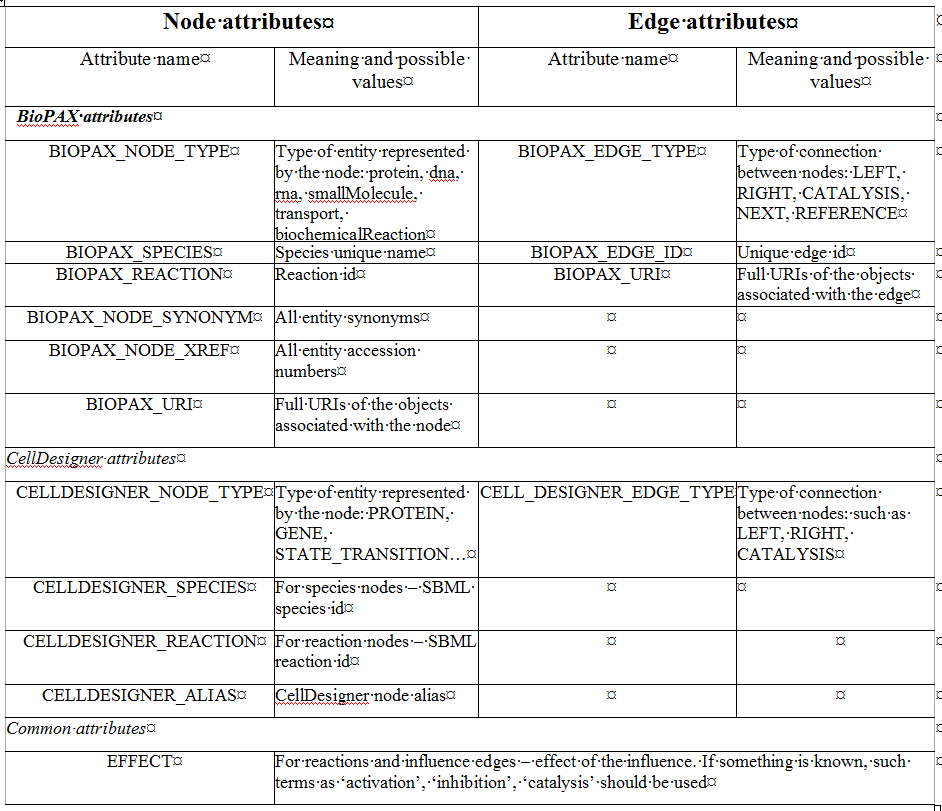
\includegraphics[width=0.8\textwidth]{graphics/Attribute_table}
\caption{All attributes of graph model used by the index}
\label{Attribute_table}
\end{figure}

\subsection{BiNoM CellDesigner and BiNoM BioPAX visual mappers}\label{CellDesigner_BioPAX_visual_mappers}
BiNoM has two built-in visual mappers supporting the visualization of the whole index or of its parts. The legend for deciphering the different types of visualization is provided in figure~\ref{BioPAX_visualizations}.
\begin{figure}
\centering
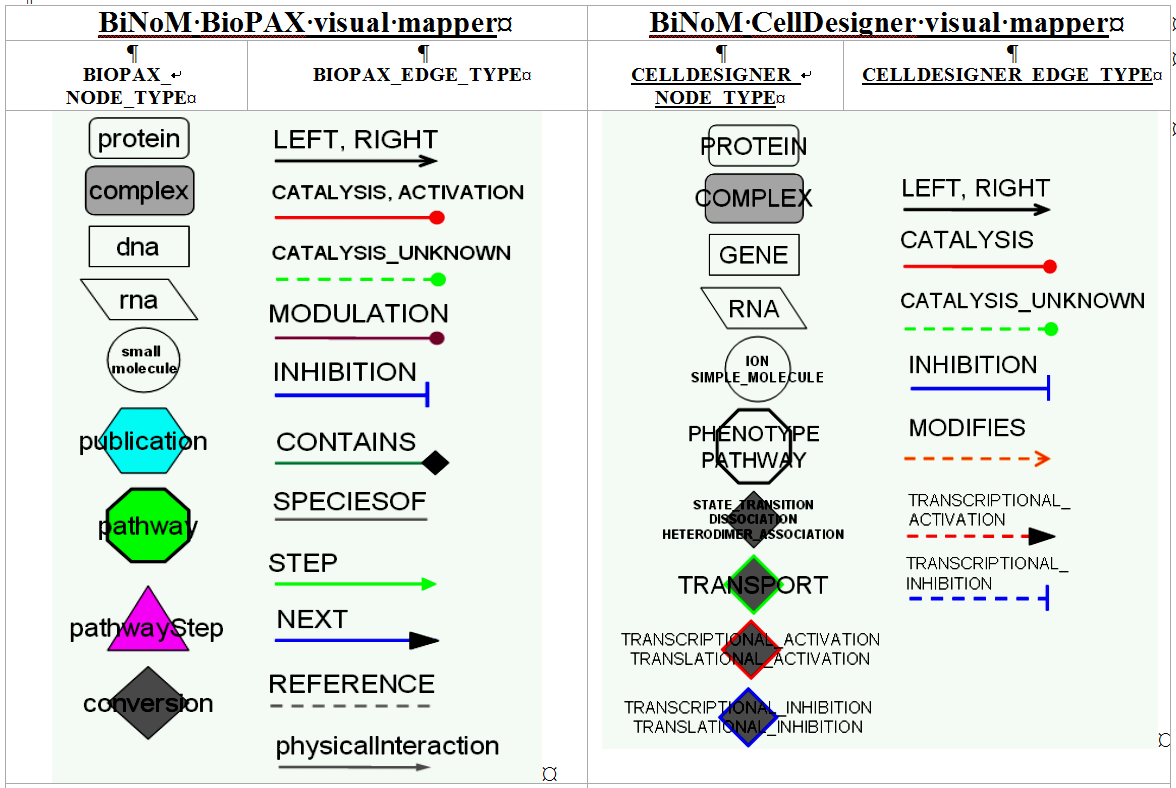
\includegraphics[width=0.8\textwidth]{graphics/BioPAX_visualizations}
\caption{Types of visualization in BioPAX and CellDesigner}
\label{BioPAX_visualizations}
\end{figure}

\subsection{BiNoM Naming Service}\label{BiNoM_Naming_Service}
When importing pathway information, BiNoM tries to generate meaningful, unique and short names for index entities. This function of the plugin is performed via BiNoM Naming Service. For proteins and other entities, the shortest available synonym is used. For genes, a ‘g’ symbol is added at the beginning of the name, and for RNAs, a ‘r’ symbol is added in order to avoid mixing genes and mRNAs with their products. If this leads to an ambiguity, it is resolved by adding a suffix specifying a unique id of the entity.\\\\
A chemical species in BiNoM is defined as a physical entity (such as protein) with some cellular localization and some (post-translational) modification (possibly none). The general template of the species label is the following:\\
Entity1\_name\textbar Modification1\textbar Modification2\textbar…: Entity2\_name\textbar Modifications...[\_active\textbar \_hmN]@compartment\\
Here, the colon symbol ‘:’ delimitates the different components of a complex if the species has several components. Optional suffixes ‘active’ or ‘hm’ describe active state of the chemical species or N-homodimer state, respectively.\\\\ Several examples of naming chemical species are presented:
\begin{itemize}
\item Naming chemical species shown in Systems Biology Graphical Notation standard figure~\ref{Names_in_SBGN_standard}
\item A conversion from CellDesigner figure~\ref{From_CellDesigner_to_Cytoscape}.
\item A conversion from BioPAX figure~\ref{Fragment_of_Apoptosis_from_Reactome}.
\end{itemize}
\begin{figure}
\centering
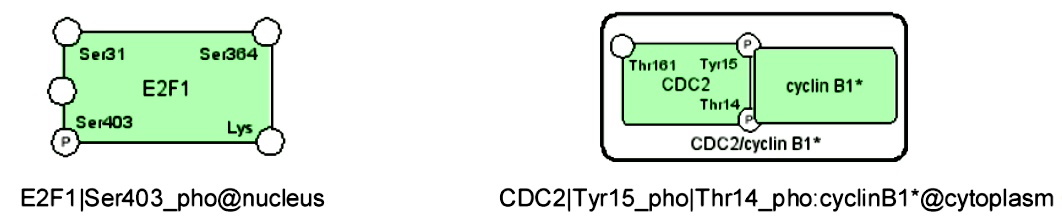
\includegraphics[width=0.8\textwidth]{graphics/Names_in_SBGN_standard}
\caption{2 examples of naming chemical species shown in Systems Biology Graphical Notation standard.}
\label{Names_in_SBGN_standard}
\end{figure}
\begin{figure}
\centering
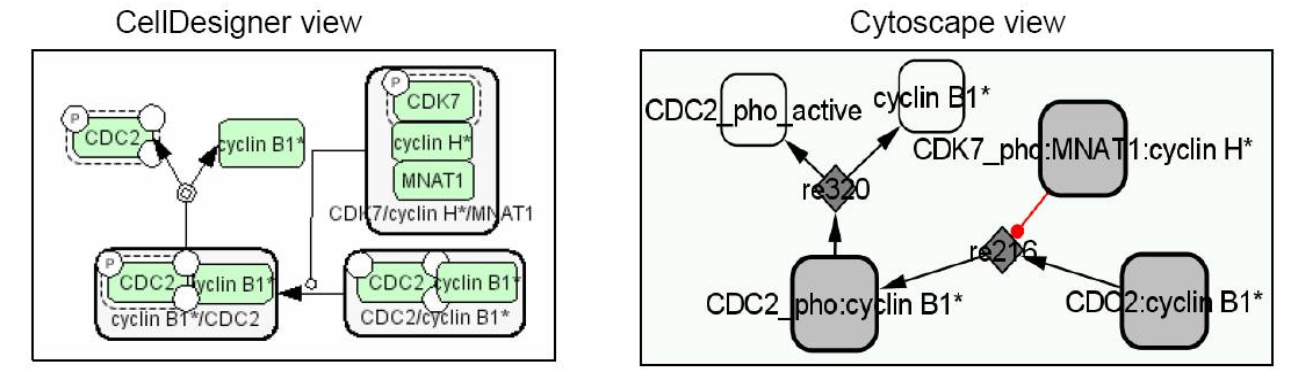
\includegraphics[width=0.8\textwidth]{graphics/From_CellDesigner_to_Cytoscape}
\caption{Conversion of a little network from CellDesigner Graphical Notation to BiNoM index representation}
\label{From_CellDesigner_to_Cytoscape}
\end{figure}
\begin{figure}
\centering
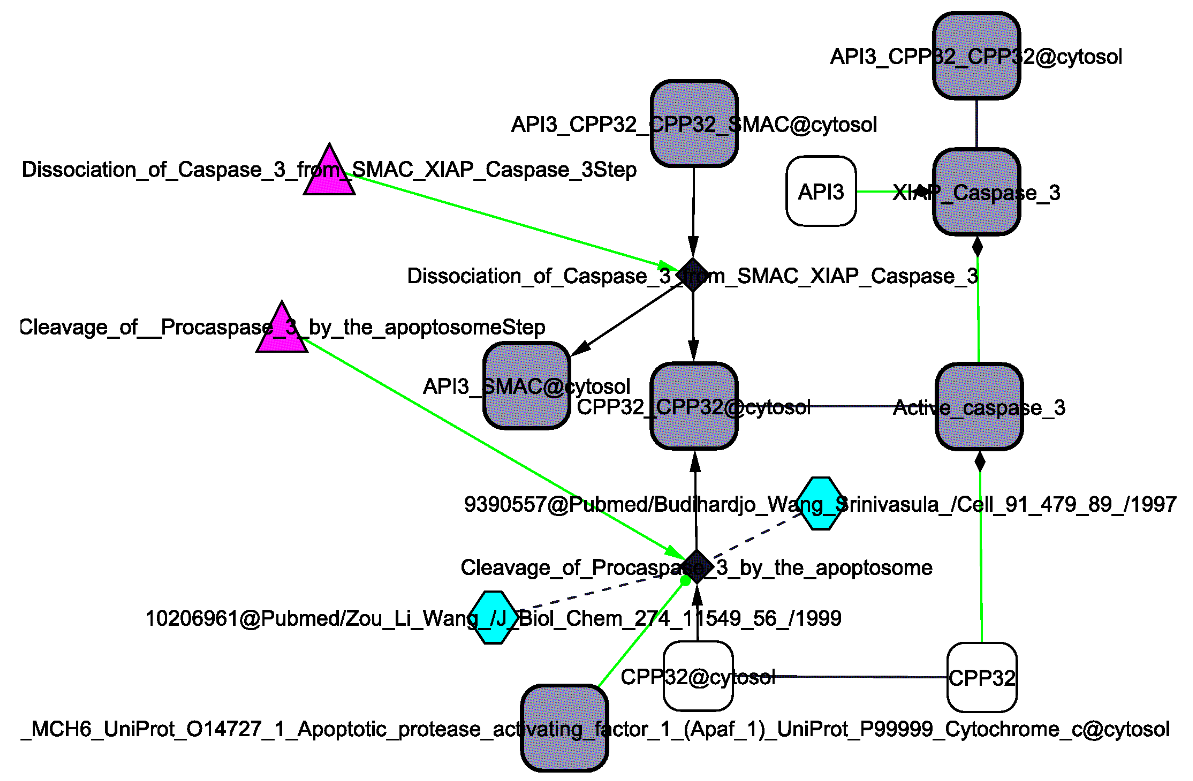
\includegraphics[width=0.8\textwidth]{graphics/Fragment_of_Apoptosis_from_Reactome}
\caption{Small fragment of BioPAX index generated for Apoptosis pathway and extracted from Reactome database}
\label{Fragment_of_Apoptosis_from_Reactome}
\end{figure}

\subsection{Standard BioPAX interfaces}\label{Standard_BioPAX_Interfaces}
BiNoM index serves as a visual connector to the content of a network file. However, with all types of relations, the index is a highly connected graph and not very insightful when represented entirely. A subgraph of the index can be extracted according to a specific purpose and used to understand a specific aspect of the pathway information. We will call interface such a subgraph of the entire index.\\\\
When importing a BioPAX file, BiNoM proposes to generate three standard BioPAX interfaces referred to as
\nopagebreak
\begin{itemize}
\item Reaction Network.
\item Pathway Structure.
\item Protein-Protein Interaction.
\end{itemize}
\subsubsection{BioPAX interface as Reaction Network}
The Reaction Network interface is a bipartite graph which contains nodes of only two types: ‘species’ and ‘reactions’. Reactants are connected to reactions through edges of type LEFT, products are connected through edges of type RIGHT. Modifier species are connected through CATALYSIS, MODULATION and other edges. See figure~\ref{BioPAX_reaction_network}.\\\\
Some BioPAX objects (catalysis, for example) are represented by edges with the corresponding BIOPAX\_URI attribute.
A chemical species node can correspond to several grouped physicalEntityParticipants, thus, it can have several BIOPAX\_URI attributes. When calling BioPAX editor, all of them will be opened.\\\\
Standard Reaction Network interface can be exported to pure SBML format (level 2) and serve as a draft for further computational modeling.
\begin{figure}
\centering
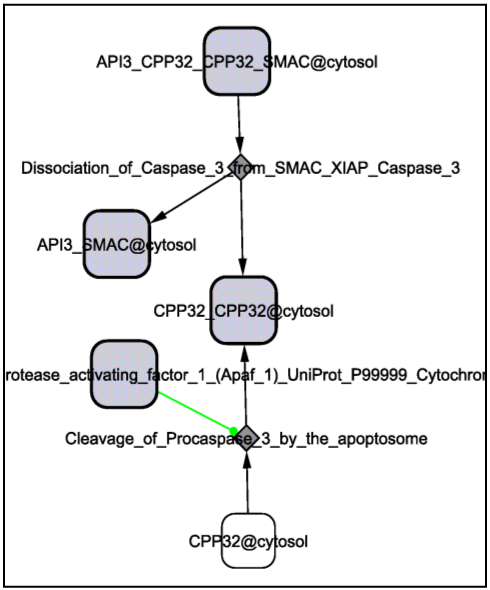
\includegraphics[width=0.8\textwidth]{graphics/BioPAX_reaction_network}
\caption{Fragment of Apoptosis from Reactome as Reaction Network.}
\label{BioPAX_reaction_network}
\end{figure}
\subsubsection{BioPAX interface as Pathway Structure}
Pathway Structure interface contains only nodes of ‘pathway’, ‘pathwayStep’ and ‘interaction’ types. The types of the edges connecting them are ‘CONTAINS’, ‘STEP’ and ‘NEXT’.  See figure~\ref{BioPAX_pathway_structure}.
\begin{figure}
\centering
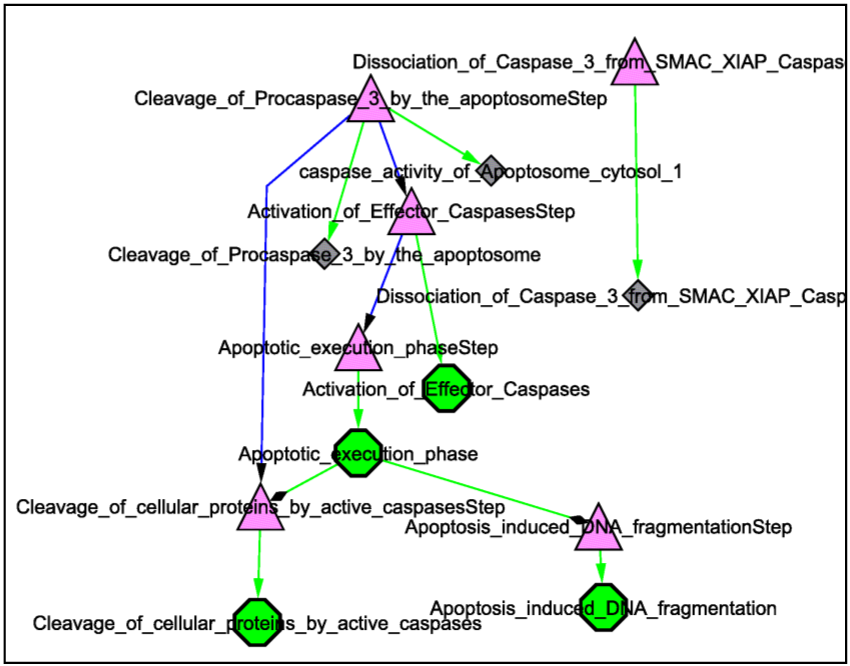
\includegraphics[width=0.8\textwidth]{graphics/BioPAX_pathway_structure}
\caption{Fragment of Apoptosis from Reactome as Pathway Structure.}
\label{BioPAX_pathway_structure}
\end{figure}
\subsubsection{BioPAX interface as Protein-Protein Interaction}
Protein-protein Interaction interface contains only entities (not chemical species) with edges of ‘CONTAINS’ and ‘physicalInteraction’ type. This interface allows to visualize the composition of complexes like the Caspase3 example of the Apoptosis pathway (left, first), or, explicit information about protein interaction with TGFB1 (left, second), as in the NetPath TGF-beta BioPAX file.  See figure~\ref{BioPAX_protein_protein_interaction}.
\begin{figure}
\centering
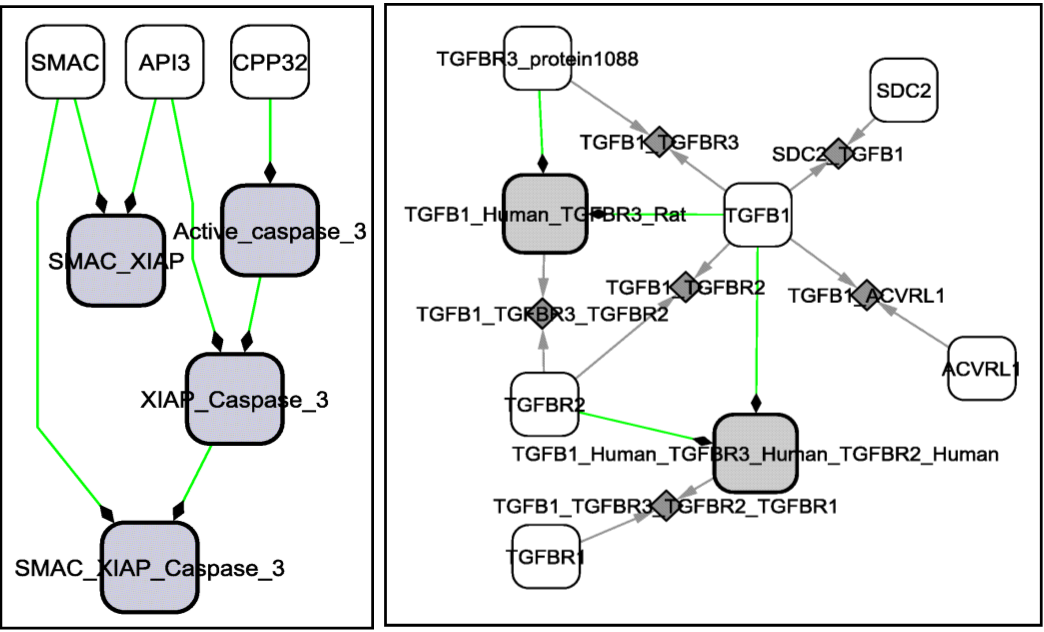
\includegraphics[width=0.8\textwidth]{graphics/BioPAX_protein_protein_interaction}
\caption{Fragment of Apoptosis from Reactome as Protein Protein Interaction.}
\label{BioPAX_protein_protein_interaction}
\end{figure}

\subsection{AIN file format} \label{AIN_file_format}
The AIN format describes a list of influences between genes, proteins, modified proteins or families. It is a table in ASCII, where the columns are separated by one tabulation (\textless Tab\textgreater) .\\\\
The first line must start with the name of each column as follows (the titles are fixed):\\
ReviewRef ExperimentRef Link ChemType Delay Confidence Tissue Comment\\
(each space corresponds to a \textless Tab\textgreater on your keyboard).
\begin{itemize}
\item For the references (ReviewRef and ExperimentRef), if one wants to include a PUBMED number, it should have the form “PMID:123456.
\item The Link column describes a connection (activation or inhibition) between two entities, like “A-\textgreater B” or “A-\textbar B”. The entities can be simply the name of a gene or a protein, but it can also be a complex (“(C:D)”), a phosphorylated protein (“(C\textasciicircum p)”) or a family. In the latter case, the family can be given explicitly by the list of all its members (“(C1,C2,C3)”) or implicitly, by un undefined name (“(C.)”), where the “.” can be replaced by any character..
\item In the other columns, if the user wishes to add more than one word in each field, the sentences need to be inserted between “…”.
\item If a field cannot be filled, a simple dot should be inserted.
\item A \# in first column makes the line comment.
\end{itemize}\
For an example of AIN format, one can open the file ExamplApop.txt in a simple text editor or in spreadsheet as EXCEL. All the information in this AIN file is translated in BioPAX format when the file is imported in Cytoscape via BiNoM.

\subsection{Modularization by shortest path clustering}\label{Agglomeration_by_shortest_path}
When only the structure of a network is known, the simplest method to agglomerate nodes in a network is to put the closest nodes together. And so modules may have the fewest links between them. This method can lead to an algorithm of modularization of an oriented network. The notion of closeness and the process of creating modules are to be clarified.\\\\
The distance between nodes is based on the length of the shortest paths and the number of occurrences if several paths are equal (the equality of the shortest path is frequent in a strongly connected network). The distance from node 1 to node 2 is generally different from distance from node 2 to node 1.\\\\
The used distance is the minimal linkage applied to the base distance, which is necessary to respect the triangular inequality. The distance between A and B is the minimum of distances from nodes in A to nodes in B and from nodes in B to nodes in A. And so, the agglomerative hierarchical clustering can be applied to build modules.\\\\
To avoid too speed increasing of clusters, they are ranked in a queue and the last created cluster is put at the end of the queue. For the same reason, nodes are sorted by in degree (sources in first). Despite of these precautions, the algorithm applied to strongly connected network gives unbalanced clusters (often a hudge cluster and several tiny clusters). So, a ceiling number of nodes in a cluster must be fixed.\\\\
The agglomerative clustering gives 1 cluster at the end, which has no interest. That’s why; these 2 stop conditions are added:
\begin{itemize}
\item The length of the shortest path between 2 clusters reaches the maximal length.
\item The number of clusters to be compared in the queue is less than 2.
\end{itemize}
The first stop condition make that too far clusters are not merged. When the last cluster to be created contains more than the maximal number of nodes, the largest cluster is excluded from the queue. Only the clusters remaining in the queue are to be compared by distance and they must be 2 or more.\\\\
The next page shows 3 examples (network inspired by toynet ). If the maximal length of the shortest paths is 1, nodes inside clusters are connected as a clique in a not oriented graph. But, if not, it may not be the case.\\\\
From a \textbf{practical point of view}, the input of ceiling number of nodes and maximal length of the shortest paths gives a set of not intersecting sub-networks. They are a partition of the network; their union is the whole network. This process is only useful for connected networks. Obviously, isolated nodes or sub-networks are not merged unless the maximal distance is infinity.

\subsection{GLOSSARY}\label{GLOSSARY}
\subsubsection{BioPAX}
BioPAX is an OWL (Web Ontology Language) document designed to exchange biological pathways. BioPAX format provides separate layers of information: information about the reactions involved in the networks along with the participants, information about the structure of the pathway, and information about the protein-protein interactions. 
\subsubsection{CellDesigner}
CellDesigner is a structured diagram editor for drawing gene-regulatory and biochemical networks. Networks are drawn based on the process diagram, with graphical notation system proposed by Kitano.
\subsubsection{BiNoM Index}
Directed labeled graph representing the objects in CellDesigner and BioPAX ontologies and their connections. Index maps only the information needed to display it and to identify the relevant information in the original CellDesigner or BioPAX files.
\subsubsection{BiNoM interface}
Part of the BiNoM index (subgraph) visually presented by Cytoscape network. There are standard interfaces (Reaction network, pathway structure, protein interaction) which can be combined to construct a user-defined interface.
\subsubsection{Optimal / suboptimal shortest paths}
Shortest paths in weighted directed graph – paths in the graph between source and target nodes with minimal sum of weights of the edges making the path. Suboptimal path is constructed by removing all edges in all shortest paths one by one and one at a time and finding the shortest path.
\subsubsection{Strongly Connected Components (SCC)}
A subgraph in a directed graph, in which there is path from any node to any node
\subsubsection{Relevant cycle}
Any cyclic path in the graph which can not be decomposed further into simpler cycles
\subsubsection{SBML}
Systems Biology Markup Language (SBML) is a standard for representing models of biochemical and gene-regulatory networks.


.